%%%%%%%%%%%%%%%%%%%%%%%%%%
% MSc Project Background Report Template
% Prof. Roger K. Moore
% University of Sheffield
% 22 March 2017
%%%%%%%%%%%%%%%%%%%%%%%%%%


\documentclass[11pt,oneside]{book}
\usepackage[margin=1.2in]{geometry}
\usepackage{setspace}
\usepackage[toc,page]{appendix}
\usepackage[none]{hyphenat} % turn hyphenation off by default
\usepackage{graphicx}
\usepackage{ragged2e}
\usepackage[section]{placeins}
\usepackage{amsmath}

\begin{document}

\frontmatter

\begin{titlepage}

% You need to edit the details here

\begin{center}
{\LARGE University of Sheffield}\\[1.5cm]
\linespread{1.2}\huge {\bfseries Reconfigurable Security for IoT Application in Handling Machine-Learning/Modelling Attacks}\\[1.5cm]
\linespread{1}

\includegraphics[width=5cm]{images/tuoslogo.png}\\[1cm]
{\Large Cheng-Wei, Tsao}\\[0.8cm]
{\large \emph{Supervisor:} Dr Prosanta Gope}\\[0.5cm]
\large A report submitted in fulfilment of the requirements\\ for the degree of BSc in Computer Science\\[0.3cm] 
\textit{in the}\\[0.3cm]
Department of Computer Science\\[2cm]
\today
\end{center}

\end{titlepage}

% -------------------------------------------------------------------
% Declaration
% -------------------------------------------------------------------

\newpage
\chapter*{\Large Declaration}

\setstretch{1.1} % set the line spacing differently if you wish, but this looks good to me. 

All sentences or passages quoted in this report from other people's work have been specifically acknowledged by clear cross-referencing to author, work and page(s). Any illustrations that are not the work of the author of this report have been used with the explicit permission of the originator and are specifically acknowledged. I understand that failure to do this amounts to plagiarism and will be considered grounds for failure in this project and the degree examination as a whole.\\[1cm]

\noindent Name: Cheng-Wei, Tsao\\[1mm]
\rule[1em]{25em}{0.5pt}

\noindent Signature: Cheng-Wei, Tsao\\[1mm]
\rule[1em]{25em}{0.5pt}

\noindent Date: November 15, 2021\\[1mm]
\rule[1em]{25em}{0.5pt}

% -------------------------------------------------------------------
% Abstract
% -------------------------------------------------------------------

\chapter*{\Large \center Abstract}
\setlength{\parskip}{\baselineskip}%
\setlength{\parindent}{0pt}%

This report investigates and provides a clear introduction on PUF(physical unclonable function),
the aim of the project and current progress. In introduction, there are thoroughly description on
PUF, reconfigurability framework and concepts corresponding to specific machine learnings
for modeling attack on PUF.

The aim of the project is to propose a novel, suitable machine learning to model PUF(physical
unclonable function) and then design a reconfigurability framework to fight against such
attack. The PUF structure is similar to a road network so machine learning related to
ETA(estimated time arrival) problem is strongly considered.

The achievements to date are having a robust understanding of PUF, reconfigurability property,
and an attempt to implement reinforcement-learning and Graph attention neural network as modeling attack. SARSALambda Q
learning has been tested on PUF but only around 60\% accuracy has been achieved. Graph attention neural network
is implemented as well, but will need to adapt to dynamic input.


% -------------------------------------------------------------------
% TOC etc
% -------------------------------------------------------------------

\tableofcontents
\listoffigures
\listoftables

\setstretch{1.1} 

\mainmatter

\chapter{Introduction}
In the rapid development of the information era, many daily events are achieved by a various of electronic devices such as computer or phones.
Those electronic devices highly rely on integrated circuits(ICs) to perform specific events. For example, bank transaction can be done by different devices,
the process contain personal data, and including usage of sensitive information. Therefore, information security like authentication, protecting confidential data
has become important in nowadays society. In order to increase security's robustness, a range of ways has been proposed. One conventional way to is by storing secret key in non-volatile memory to encrypt sensitive data with it,
and use asymmetric cryptography to authenticate the device \cite{Reference3}. However, the implementation process of cryptography is expensive, especially on resource-constraint device, and the device is still vulnerable to invasion attack. Ideally, devices should be able to handle challenging problems corresponding to energy consumption, 
computational power and the ability to fight against cyber attack. \par

PUF(physical unclonable function) has the ability to deal with these challenges. It does not store secret in non-volatile memory, instead, the volatile secret is derived from devices' physical characteristics \cite{Reference3}.
This is based on the inevitable random variation in ICs manufacturing process, which leads to the fact that no two IC have exact same physical characteristic. For example, each ICs has unique delay sequences in the transistors and wires.
With this property, PUF does not require lots of computational power and is cost-effective because no need to implement cryptographic operation, which works particular well on
resources-constraint devices such as RFID. Also, the attacker needs to perform attack when the device is on, which significantly increase the difficulty. As for invasion attack, 
the attacker needs to have the exact information of its unique physical characteristics to successfully derive secret. Overall, PUF provides another interesting way for reinforce security.

\section{Aims and Objectives}
The objectives split into two parts for this project. In the first stage, propose a novel machine learning to modeling different PUF(physical unclonable function)
behavior, so predict the response from a given PUF when given challenge bits. For example, considered the simplest PUF which is arbiter PUF, its operation to create a response is to
input a challenge bits(binary), and two signals will go thorough the multiplexers in the PUF structure depend on the value of it. Consequently response a binary bit
that will indicate which signal is faster. Therefore, the machine learning for modeling will be related to ETA(estimated time arrival) problem since the structure of PUF is similar to a road network. 
For instance, traveling through each multiplexer is similar to traveling through each road segment, and both of them have delay to affect the time of arrival. Overall the first stage is to design a machine learning
consider these concepts. In the second stage, design a reconfigurability framework to fight against such modeling. In detail, evaluate the machine learning by insert noise in PUF or experiment on OPUF(one-time-PUF) which
contain reconfiguration process that can alleviate modeling attack.

\section{Overview of the Report}
The remaining of the paper will organize as follow. Chapter 2 provide literature survey of the concept of PUF, including PUF's properties, detailed circuit structure and operational process, 
exist modeling attack with experiment results, reconfigurability framework and application in life. Relative machine learning idea will be discuss as well. Chapter 3 describe the aim and objectives for the project
, gives in-depth analyzes how the project will be evaluated, the tests and experiments that support this. Chapter 4 demonstrate the current progress on the project. Chapter 5 provide brief
summary on the main achievements with a well organized future plan for the project.

\chapter{Literature Survey}

\section{The PUF concept}
The simplest sentence to describe PUF is "A PUF is an object's fingerprint" \cite{Reference4}. The fingerprint can represent a specific human in the world, such as the PUF can represent
an object. The fingerprint is inherently created when people was born, and the so does PUF, which is inherently exist in an object according to unique manufacturing random variation \cite{Reference4}.
With the representation and inherent property, the fingerprint and the PUF is said to be unclonable since it is impossible to control and predict human's fingerprint. This is an important concept for PUF. \par

This intrinsic property can be extract from chip which has PUF circuit existed inside \cite{Reference2}. The way PUF works is by entering a certain length of bits(so called challenge) into the PUF, and it will
generate another specific length of bits(so called response). According to the property of PUF that was discuss above, it is impossible to find two different PUF that will produce the same response when entering same challenge(See Figure \ref{fig:figure1}).
\begin{figure}[htp]
\centering
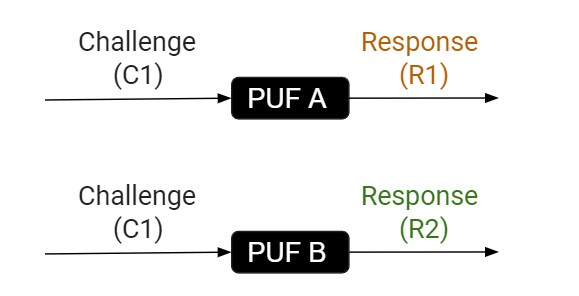
\includegraphics[width=8cm]{figures/figure1.jpg}
\caption{Different PUF that generate different response when input same challenge}
\label{fig:figure1}
\end{figure}

\section{Weak and strong PUF}
PUF can be classified into two categories, weak and strong PUF according to the strength of PUF. The strength of PUF indicate the number of challenge response pairs(so called CRPs) can be generate 
from the PUF \cite{Reference1}. The higher numbers of the CRPs can a PUF generate, the better strength it has. Generally, if increasing the size of the PUF leads to a linear increase in the number of CRPs, it is consider weak PUF. 
On the other hand, if increasing the size of the PUF leads to a exponential increase in the number of CRPs, it is consider strong PUF.\par

For the weak PUF, it represent the PUF that has smaller set of CRPs. While it is impossible to 
create a clone of PUF, but with small set of CRPs, this will allow attacker to record all the CRPs when attacker has physical access to PUF \cite{Reference1}. With the knowledge of CRPs, attacker can easily provide the corresponding
response to challenge as like they have a clone(See Figure \ref{fig:figure2}). The weak PUF can be use for authentication and key storage. However, since weak PUF's CRPs can be fully access, ensure having a secure environment and whether the original PUF is being evaluating is relatively important \cite{Reference1}.
\begin{figure}[htp]
    \centering
    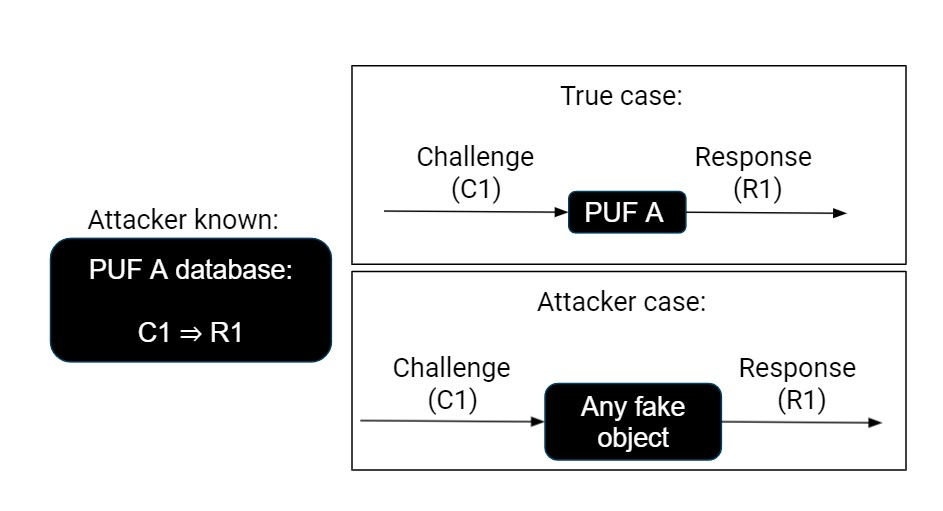
\includegraphics[width=10cm]{figures/figure2.jpg}
    \caption{Attacker can perform same behavior as Weak PUF when have fully access to CRPs and not under secure environment}
    \label{fig:figure2}
    \end{figure}

For strong PUF, means the number of CRPs is significantly large that even attacker get access, having throughout knowledge of CRPs is impossible. While the number of CRPs is so large,
and the CRP are randomly selected in usage, the probability that attacker has knowledge about the CRP currently using is small. In addition, each CRPs that is used once will 
be discarded(See Figure \ref{fig:figure3}) so even if attacker recorded certain CRPs, also called eavesdropped, they will not be able to put them into use. The strong PUF can also be use for authentication but do not need to protect CRPs
as serious as weak PUF.

\begin{figure}[htp]
    \centering
    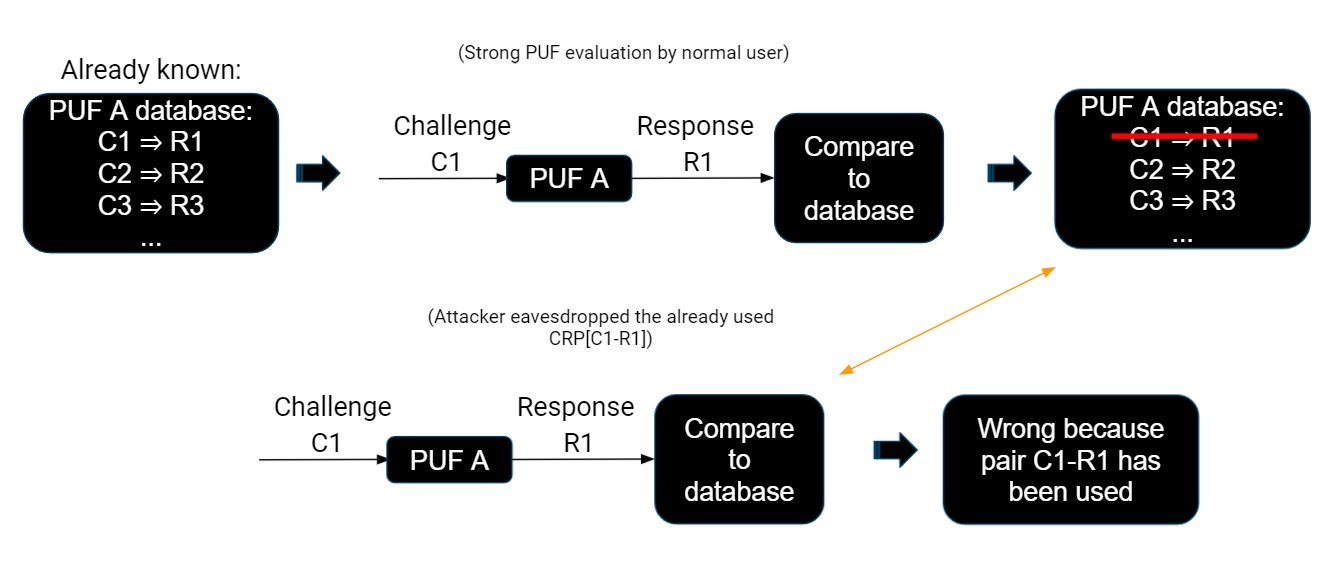
\includegraphics[width=15cm]{figures/figure3.jpg}
    \caption{The attacker eavesdropped CRP that has been used can not successfully validate in next evaluation for strong PUF}
    \label{fig:figure3}
    \end{figure}

\section{Authentication}
One of the application of PUF is authentication. As discuss in Chapter 1's introduction, PUF does not require huge computational power and are cost effective, so it is suitable for many devices,
especially the resources-constraint devices. The PUF's authentication included two stages, enrollment and authentication stage. In the enrollment stage, the company possess the PUF, so
company can connect server to PUF and sent lots of challenges along with recording the CRPs into the database \cite{Reference2} (See Figure \ref{fig:figure4}).

\begin{figure}[htp]
    \centering
    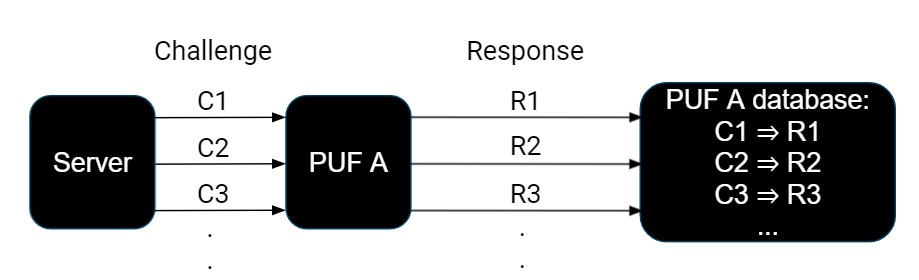
\includegraphics[width=8cm]{figures/figure4.jpg}
    \caption{Enrollment stage in PUF authentication}
    \label{fig:figure4}
    \end{figure}

After recording all the CRPs, the company can now implement PUF on electronic devices.
In the authentication stage, the server sent arbitrary challenge to the devices that contain PUF while the device will return response. Afterward, the server compare the response from the device with the database, 
if the challenge and response pair exist in the database, the device is valid \cite{Reference2} (See Figure \ref{fig:figure5}). A life example will be banking card.

\begin{figure}[htp]
    \centering
    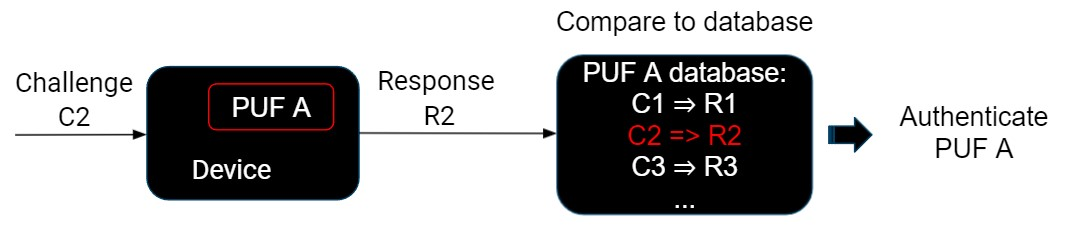
\includegraphics[width=8cm]{figures/figure5.jpg}
    \caption{Authentication stage in PUF authentication}
    \label{fig:figure5}
    \end{figure}

\section{Arbiter PUF and XOR arbiter PUF}
There are many different types of PUF such as arbiter PUF, ring oscillator PUF, lightweight PUF, etc. In this paper, arbiter PUF and its mutation will be introduced in detail. The general idea of
the arbiter PUF is comparing the transition speed for two electrical signal in the PUF's structure(See Figure \ref{fig:figure6}). The arbiter PUF's structure contains a numbers of 
multiplexers and a arbiter(mostly D flipflop), and two multiplexers will combined into a switching box \cite{Reference3}. Look at Figure \ref{fig:figure6}, when enter a challenge bits, apply each challenge bit to a switching box, bit 1 indicate the upper and lower signal will switch 
while bit 0 indicate the two signals remain unchanged in each switching box. This will eventually form paths for the signals. Then the signals start transferring, the time arrived at the arbiter for two signals 
is different since each multiplexer and wire has unique delay. The arbiter will determine which path is faster and based on that response a binary bit, if upper path is faster, the response is 1, 
otherwise the response is 0. \par

The arbiter at the end is always fair, which will not favor any one of the path. Even there exist bias, a simple solution of adding a delay in the structure can solve the problem. For example, if the arbiter favor the lower path,
by adding a delay to upper path, it can has a head start. By looking at the Figure \ref{fig:figure6}, it is clear that the CRPs will be exponential. Assuming there are n switching boxes, two possible cases in each switching box, so the 
number of CRPs is $2^{n}$, which indicate the arbiter PUF is a strong PUF. Arbiter PUF can also return longer response by input K different challenges and get a K bits response.

\begin{figure}[htp]
    \centering
    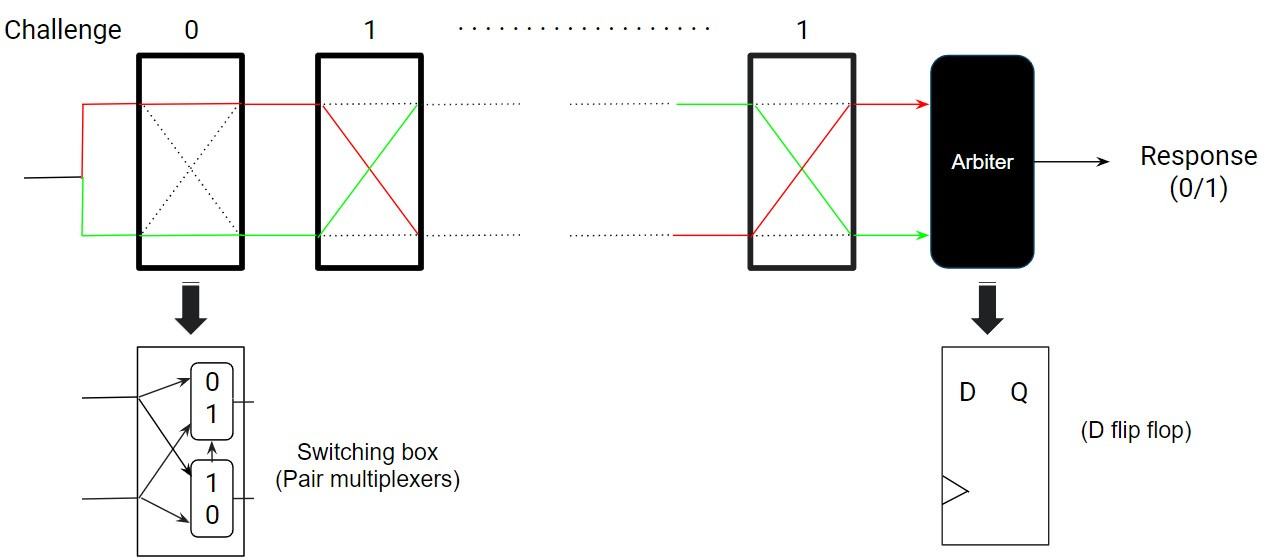
\includegraphics[width=12cm]{figures/figure6.jpg}
    \caption{Arbiter PUF structure}
    \label{fig:figure6}
    \end{figure}

The normal arbiter PUF is vulnerable to modeling attack, the propose of XOR arbiter PUF is to increase the robustness of arbiter PUF. The basic concept is to integrated multiple parallel arbiter PUF, given same challenge to each arbiter PUF and XORed each response to produce final response(See Figure \ref{fig:figure7}) \cite{Reference5}.
According to simulation, in book \cite{Reference4} provides the XOR arbiter PUF will have nonlinearity property that makes it harder to model.

\begin{figure}[htp]
    \centering
    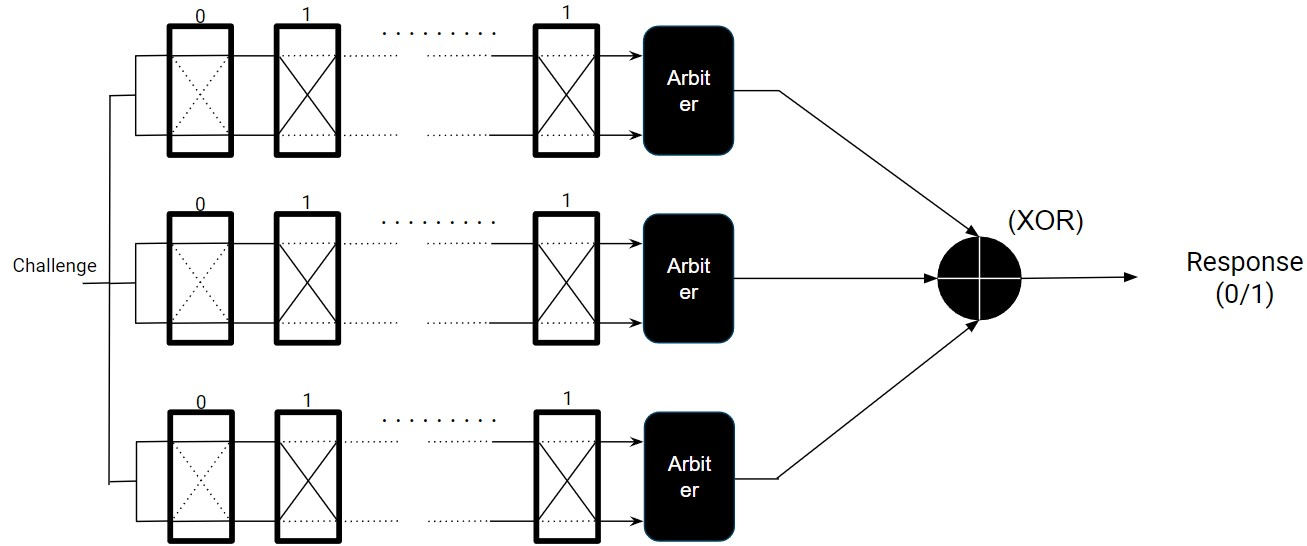
\includegraphics[width=12cm]{figures/figure7.jpg}
    \caption{XOR arbiter PUF structure}
    \label{fig:figure7}
    \end{figure}

\section{Modeling attack on PUF}
Many different threat can perform on devices, such as eavesdropped, gain access to the memory that store secret keys. For PUF, the main threat is that attacker can use technique 
like machine learning to simulate the behavior of CRPs(so called modeling), which means even without the devices, attacker can still response correctly when a challenge is 
provided. Take arbiter puf as example, assume an arbiter PUF with i switching box, and the challenge apply to each switching box is c[i]. The two signal travel through the 
the path determine by challenge, and arrive at the arbiter in different time because of the delay in each component. The final response depend on the sign of final delay 
difference:
\begin{equation}
    r =\begin{cases}
    1, & \text{if $\Delta c<0$}.\\
    0, & \text{otherwise}.
    \end{cases}
\end{equation}
which the delay difference is calculated by subtract the upper path with lower path's delay. The final delay difference $\Delta c$ can represent as $w^{T}\Phi$, where $w^{T}$ is 
a weight vector that represent delays for the components in PUF, and $\Phi$ is the applied i bits challenge \cite{Reference5}. $w^{T}\Phi = 0$ will provide a hyperplane that separate the space for $\Phi$, one side of the hyperplane are predict as having response 1, the other side of the hyperplane
are predict as having response -1. In conclusion, the correct hyperplane indicate the good prediction of PUF. Machine learning such as logistic regression can play the role well. The modeling result for a arbiter PUF with 64 switching boxes, 
by using the logistic regression can get a good performance of 99.9\% in very short time with 18050 training CRPs \cite{Reference6}.

For the XOR arbiter PUF, it is also possible to use logistic regression to predict the behavior but will be harder.

\section{Reconfigurability of PUF}
In order to alleviate the problem that PUF is vulnerable to modeling attack, reconfiguration property embedded on PUF has been proposed. For example, the one-time-PUF(so called 
OPUF), the general idea is that the its configuration alter after every authentication session, which means CRPs behavior of the PUF is changed and invalidate the modeling attack. This is based on the
forward unpredictability and backward unpredictability properties that OPUF possess \cite{Reference7}. In Figure \ref{fig:figure8} shows the concept of forward unpredictability and backward unpredictability.
The orange line represent the forward unpredictability, which will ensure the responses collected before the reconfiguration process is invalid afterward. As for the blue line, 
which represent backward unpredictability, it will ensure the pattern observed by attacker using modeling attack on PUF' is invalid for predicting the PUF before reconfiguration process. 
In this case, assume an attacker are performing a modeling attack on the PUF, and required certain amount of CRPs to gain proper prediction. However, the OPUF's structure keep changing every execution, which means the CRPs 
behavior is changing, so the modeling attack will can't be up to date or do mot have time to collect enough CRPs.
\begin{figure}[htp]
    \centering
    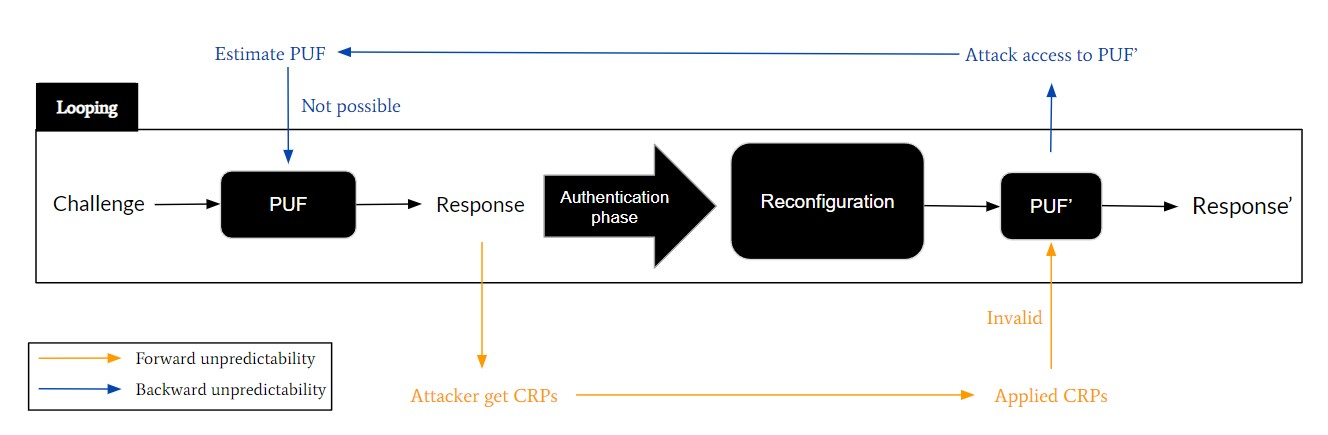
\includegraphics[width=14cm]{figures/figure8.jpg}
    \caption{Concept of forward unpredictability and backward unpredictability}
    \label{fig:figure8}
    \end{figure}

DPUF can be consider as an example for creating the OPUF, it is build up with bit cells which contain capacitors and transistors, each cell store information of value 0 and 1. However, these component will leak 
electrical signals every period of time, which means the behavior might be eavesdropped \cite{Reference7}. Therefore performing reconfiguration process every period of time is effective. The reconfigurability can be shown in Figure \ref{fig:figure9}, by varying parameters
such as refresh-pause interval and the memory block, where the former can cause random bit flip in the cells while the latter store final response in an random memory block 
which will alter every period of time, PUF can present unpredictable behavior that prevent from attacker perform modeling attack.

\begin{figure}[htp]
    \centering
    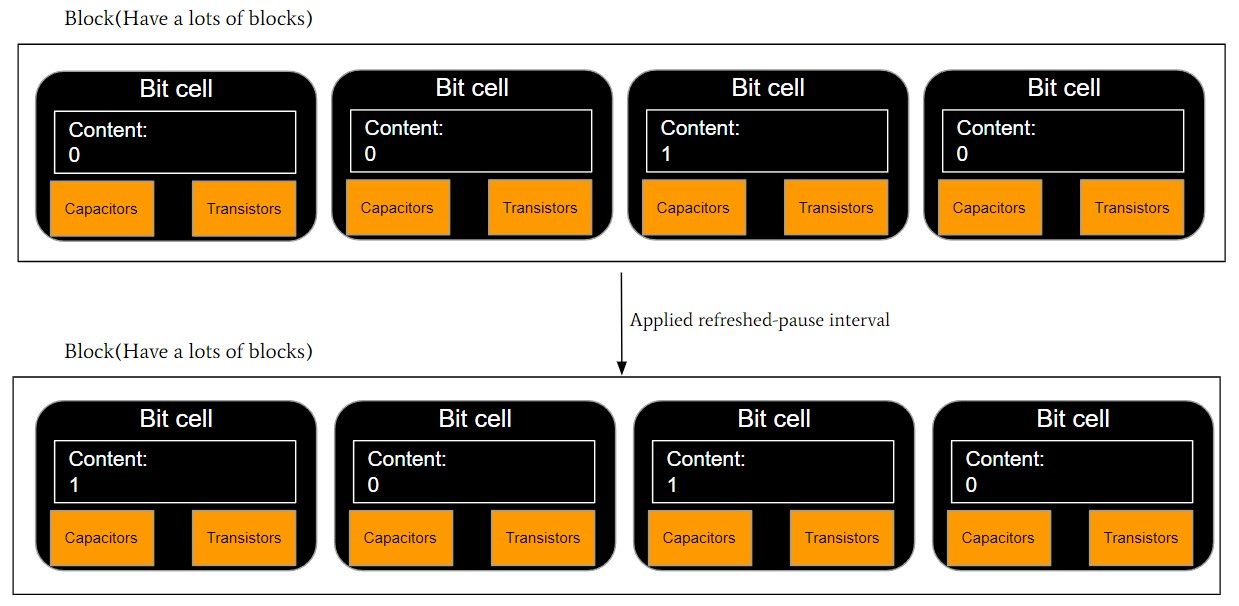
\includegraphics[width=10cm]{figures/figure9.jpg}
    \caption{Reconfigurability framework of DPUF}
    \label{fig:figure9}
    \end{figure}

\section{Summary}

How this concept of PUF can help my investigation.....etc...

\chapter{Analysis}
Overall, total two objectives are required for the project. In the first part, propose a novel machine learning to modeling different PUF(physical unclonable function)
behavior, in particular arbiter PUF and XOR arbiter PUF. In the second part, consider reconfigurability like adding noise, one-time-PUF to resilient against the modeling attack
proposed in part one.

\section{Project Aims and Evaluation}
The aims for part one are that the machine learning for modeling should be related to ETA(estimated time arrival) problem or the one people haven't used for modeling
PUF. Moreover, reconfigurability need to be considered when proposing the modeling attack while knowing the PUF can escape from it by changing CRPs behaviors in part 
two. Therefore, the machine learning should ideally adapt to the changing behavior of CRPs or the PUF. For example, unsupervised learning can be a good way since it can 
deal with unseen data. To evaluate the work, an overall accuracy of the modeling are expected to be around 90\% and take short time like the logistic regression in 
paper \cite{Reference6}.

The aims for part two are proposing a reconfigurability framework for the modeling attack in part one. Two different reconfigurability will be implemented. First, add intentional
noise to PUF's response during authentication phase to disturb the modeling attack \cite{Reference8}. The basic idea is shown in Figure \ref{fig:figure10}, assume database has stored PUF's CRPs and provide a challenge c
to PUF in authentication phase. The PUF return a response r', and add noise e with r'. Then e and r' compose helper data h and send back to verifier, where $h = r'\oplus e$. The verifier can reproduce $r'\oplus e$  
with r and h if r and $r'\oplus e$ is similar. Last, both verifier and user create their own hashtag and compare to check if authenticate. In this case, attacker only access to c and $r'\oplus e$, which the modeling
will not be accurate unless the attacker's model response is closed enough to r'. To evaluate the work of adding intentional noise, the modeling attack proposed in part one should have reasonable accuracy drop and the authentication will still work 
though noise is added.

\begin{figure}[htp]
    \centering
    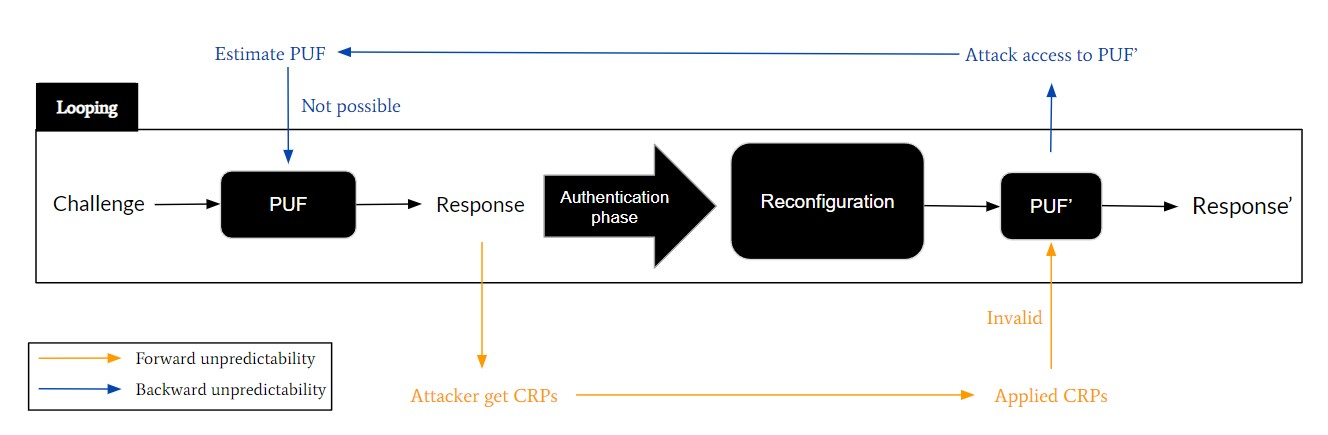
\includegraphics[width=14cm]{figures/figure8.jpg}
    \caption{Add noise to PUF's response during authentication phase}
    \label{fig:figure10}
    \end{figure}

Second, implement protection which referring to OPUF to change the behavior of CRPs and prevent modeling attack. With control of parameter like 1. Refreshed-pause timing 2. Allocating memory block, 
the project will examinate the result of the protection. For example, look at the accuracy and time consumed when apply the modeling attack in part one.





\chapter{Progress}

\section{Project progress}
The project has two parts, currently, the progress is at the point of discovering and implementing machine learning for modeling the arbiter PUF. Methods such as reinforcement learning
and graph attention neural network(so-called GAT) were used. First, the type of reinforcement learning that was implemented is the SARSALambda Q learning \cite{Reference9}. The general idea is that an agent will 
explore the environment with a final goal by randomly choosing actions space and recording the rewards. 

Assuming Figure \ref{fig:figure11} is the PUF environment, a red and green circle is the starting point for top path and bottom path, each black rectangle represents a multiplexer with unique delay and the yellow 
circle is the goal. There are three actions: going up, going down and going straight. The reward of the multiplexer is determined by the delay, the bigger the delay, the smaller the reward, vice versa. In the training phase, 
the agent will travel through different combinations of multiplexers and construct a Q table(See Table \ref{tab:table1}) by collecting rewards on multiplexers. The final goal for the agent is to find the route with 
the lowest delay. After the training, when selecting a CRPs, and inputting the challenge to the agent, ideally, the agent can calculate, compare two paths' reward and reply the correct response. For example, assume 
a challenge 00001 has response 1(which means the bottom path is faster), the calculation operation is:
\begin{equation}
    Challenge(00001) =\begin{cases}
    0.082+0.008+0.041+0.002+0.07 = 0.203, & \text {Top path: 1,3,5,7,10}.\\
    0.022+0.415+0.222+0.555+0 = 1.214, & \text {Bottom path: 2,4,6,8,9}.
    \end{cases}
\end{equation}

\begin{equation}
    0.203 < 1.214, \text { return response: 1}.
\end{equation}
In general, the route with lower delay will have a higher reward, on the other hand, the route with higher delay will have a lower reward. If the agent can predict with high accuracy, the arbiter PUF's CRPs pattern can say to 
be successfully modelled. However, the accuracy for this modeling is around 60\% - 69\%, which is not a satisfying result. The problem can be the following: not providing enough features, the exploration does not 
cover every possible route, etc.

\begin{figure}[htp]
    \centering
    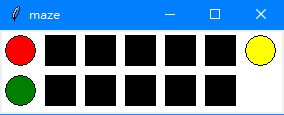
\includegraphics[width=6cm]{figures/figure11.jpg}
    \caption{SARSALambda Q learning example environment}
    \label{fig:figure11}
    \end{figure}

\begin{table}[ht]
    \center
    \begin{tabular}{c|ccc}
    Multiplexer & go up & go down & go straight\\
    \hline
    1 & 0.000 & 0.028 & 0.082\\
    2 & 0.094 & 0.000 & 0.022\\
    3 & 0.000 & 0.357 & 0.008\\
    4 & 0.009 & 0.000 & 0.415\\
    5 & 0.000 & 0.181 & 0.041\\
    6 & 0.042 & 0.000 & 0.222\\
    7 & 0.000 & 0.641 & 0.002\\
    8 & 0.003 & 0.000 & 0.555\\
    9 & 0.000 & 0.070 & 0.000\\
    10 & 0.000 & 0.000 & 0.131\\
    \end{tabular}
    \caption{Q table for example environment}
    \label{tab:table1}
    \end{table}

As for the GAT \cite{Reference10}, the basic idea of the GAT is that each node aggregate the neighbours’ features based on adjacency matrix, adjacency attention value then update each node's features. 
The updated features will insert into the neural network and perform the classifying task. In order to reach high accuracy, the main task for the GAT is to update the adjacency attention matrix to
reasonable value.

For a detail example, look at Figure \ref{fig:figure12}, which is a arbiter PUF structure. Assume each node in Figure \ref{fig:figure12} represent a multiplexer, and has node feature $f1,f2,f3,f4$. If input a 
challenge 00, a one way relation is defined: 
$m3 \rightarrow m1$, $m4 \rightarrow m2$, including self-loop, and the adjacency matrix can be constructed(See 4.3). 
\begin{equation}
    \begin{blockarray}{ccccc}
    M1 & M2 & M3 & M4\\
    \begin{block}{(cccc)c}
        1 & 0 & 0 & 0 & M1\\
        0 & 1 & 0 & 0 & M2\\
        1 & 0 & 1 & 0 & M3\\
        0 & 1 & 0 & 1 & M4\\
    \end{block}
    \end{blockarray}
    \label{matrix}
\end{equation}

\begin{figure}[htp]
    \centering
    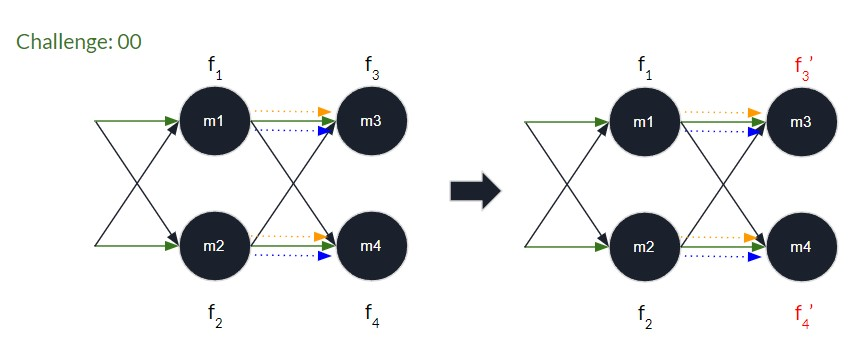
\includegraphics[width=16cm]{figures/figure12.jpg}
    \caption{GAT aggregation}
    \label{fig:figure12}
    \end{figure}

In article \cite{Reference10}, there are four steps to aggregate the features of each node. The first step, add a weight matrix $\mathcal{W}$ to gain enough expressive power to transform the features into higher-level features:
\begin{equation}
    n_i = \mathcal{W}f_i
\end{equation}

The second step, calculate a un-normalized attention value between every two nodes(i and j), but only consider nodes that is neighbor of i($j \in N_i$), where $N_i$ is the neighbor of node i that can be observed in 
adjacency matrix(See 4.3). First, concatenates the features of the two nodes(symbol $\Vert$ represent concatenation), then perform a dot product with a trainable weight vector a, and applies a LeakyReLU at last:

\begin{equation}
    c_{ij} = LeakyReLU(\overrightarrow{a}^T(n_i \Vert n_j))
\end{equation}

The third step, apply Softmax function to normalize:
\begin{equation}
    \alpha_{ij} = \frac{exp(c_{ij})}{\sum_{k \in N_i}  exp(c_{ik})} 
\end{equation}

The fourth step, aggregate the updated features from neighbors to current node, which consider the attention matrix:
\begin{equation}
    f_i^{'} = \sigma (\sum_{j \in N_i} \alpha_{ij}n_j)
\end{equation}

After updating every node's features, concatenates the node features of top path($f_1^{'}+f_3^{'}$)and bottom path($f_2^{'}+f_4^{'}$), and insert into a classify layer. Next, compare the output with ground fact
(response of the challenge) and update the trainable parameter to increase the modeling accuracy. Ideally, the adjacency matrix will keep updating according to different input challenges, and the GAT will be able to 
learn the pattern after looking at many CRPs. However, there is doubt that whether the GAT support dynamically changing adjacency matrix, so this idea is not done yet.






\chapter{Conclusions}

\section{Summary of the project and project Plan}
Currently, the project is still at the stage of designing modeling attack, which is the first part of objectives mentioned in Chapter 1. As stated in Chapter 4, reinforcement learning and GAT still suffer from implementation problems. For the short term goal, in the next few weeks till 12/22's meeting,
the main task is to successfully implement modeling attack mentioned in Chapter 4 or other methods that can achieve prediction accuracy higher than 80\%. The XGBoost was a new idea to try if both the previous machine learning fail to implement or model the arbiter PUF. 
However, more research on XGBoost was required. In addition, investigate more about pypuf, and try fully understand the paper \cite{Reference11}, then prepare a presentation for 12/22's meeting.


In the long term, after the modeling attack is implemented, start on designing a reconfigurability framework to prevent the attack. The framework that was mentioned in Chapter 2 and Chapter 3 will be considered. The framework
is expected to be completely implemented at the end of March 2022 so there will have enough time for testing and writing dissertation.


\bibliographystyle{acm} 
\bibliography{reference} 

\begin{appendices}
\chapter{An Appendix of Some Kind}


\chapter{Another Appendix}

Lorem ipsum dolor sit amet, consectetuer adipiscing elit. Aenean commodo ligula eget dolor. Aenean massa. Cum sociis natoque penatibus et magnis dis parturient montes, nascetur ridiculus mus. Donec quam felis, ultricies nec, pellentesque eu, pretium quis, sem. Nulla consequat massa quis enim. Donec pede justo, fringilla vel, aliquet nec, vulputate eget, arcu. In enim justo, rhoncus ut, imperdiet a, venenatis vitae, justo. Nullam dictum felis eu pede mollis pretium. Integer tincidunt. Cras dapibus. Vivamus elementum semper nisi. Aenean vulputate eleifend tellus. Aenean leo ligula, porttitor eu, consequat vitae, eleifend ac, enim. Aliquam lorem ante, dapibus in, viverra quis, feugiat a, tellus. Phasellus viverra nulla ut metus varius laoreet. Quisque rutrum. Aenean imperdiet. Etiam ultricies nisi vel augue. Curabitur ullamcorper ultricies nisi. Nam eget dui. Etiam rhoncus. Maecenas tempus, tellus eget condimentum rhoncus, sem quam semper libero, sit amet adipiscing sem neque sed ipsum. Nam quam nunc, blandit vel, luctus pulvinar, hendrerit id, lorem. Maecenas nec odio et ante tincidunt tempus. Donec vitae sapien ut libero venenatis faucibus. Nullam quis ante. Etiam sit amet orci eget eros faucibus tincidunt. Duis leo. Sed fringilla mauris sit amet nibh. Donec sodales sagittis magna. Sed consequat, leo eget bibendum sodales, augue velit cursus nunc.

\end{appendices}

\end{document}
